\section{Verifikasjon og test} 
\label{sec:verifikasjon}
%\textit{Her dokumenteres hvordan systemet er testet. Resultat av test og drøfting av potensielle forbedringer. Det er viktig å få med at systemet eller deler av systemet virker eller ikke virker. Dersom det er mulig å tallfeste \textbf{hvor godt} systemet virker, er det bra.}

\textbf{Om du har testet et systemkrav er det mulig å bruke ID-en fra kap 3.8.} \todo{Denne må fjernes før vi leverer}


\subsection{Kamera}\label{sec:verifikasjon:kamera}

Systemkrav \idref{id:kamera} er oppfylt ut fra spesifikasjonene oppgitt av FLIR. 


\subsubsection{Rekkevidde}\label{sec:verifikasjon:rekkevidde}
Kamera har rekkevidde opp mot 30m, og kan klare å se fugler i høyder over dette. 
I \autoref{fig:verifikasjon:bilde_fugl} kan vi se et eksempel på et bilde av en fugl mot skyfri himmel. 
Det var hovedsaklig måker som var til stede under testingen, og disse kan man tydelig se med kamera i høyder opp til 30m. 
Dette er estimert ved å sammenligne med høyden til bygninger i området. 
Det er stor usikkerhet i høyden fuglene ble observert, men fra testingen er det ikke urealistisk at man kan observere større fugler i høyder rundt 40-50m. 
Dette betyr at systemet potensielt kan oppfylle systemkrav \idref{id:rekkevidde} gitt gode forhold, men problemet med testingen av rekkevidde var mangel på måleutstyr slik at man ikke kan fastslå nøyaktig høyde for de fuglene som var synlig eller ikke synlig på bildene.
Dette gjør at systemkrav \idref{id:rekkevidde} ikke er fulstendig oppnådd, og fører videre til at systemkrav \idref{id:temperatur} ikke er oppnådd grunnet vanskelige verifikasjon av høyde og størrelse.\todo{Det kan da være oppnådd selvom det ikke er verifisert på grunn av vanskelig å teste? Omformulere?}


\begin{figure}[H]
    \centering
    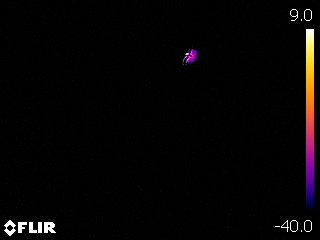
\includegraphics[width=.5\textwidth]{verifikasjon-test/Kamera/FLIR0059.jpg}
    \caption{Her kan vi se et bilde av en måke tatt med kameraet. Denne fuglen var ca. 10-20m oppe i lufta. Bildet er slått sammen av et vanlig bilde og et termisk bilde med FLIR sin programvare.}
    \label{fig:verifikasjon:bilde_fugl}
\end{figure}

\subsubsection{Værforhold}\label{sec:verifikasjon:kamera:værforhold}

Kameraet ble testet mot åpen himmel og mot skyer. 
I \autoref{fig:verifikasjon:kamera_skyfri} kan vi se et eksempel på hvordan et bilde ser ut med kameraet rettet mot åpen himmel uten fugler i bildet. 
Dette gir lite støy å filtrere bort, som man tydelig kan se fra bildet. 
Dette gir relativt enkle bilder for filtrering, som vi for eksempel kunne se i \autoref{fig:verifikasjon:bilde_fugl}. 


\begin{figure}[H]
    \centering
    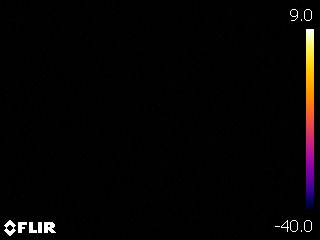
\includegraphics[width=.5\textwidth]{verifikasjon-test/Kamera/skyfri.jpg}
    \caption{Her kan vi se et bilde tatt med kameraet rettet mot en skyfri himmel. Vi kan se at det ikke reflekteres noe IR-stråling fra himmelen.}
    \label{fig:verifikasjon:kamera_skyfri}
\end{figure}

Derimot blir oppgaven mye mer krevende dersom man har skyer på himmelen. I \autoref{fig:verifikasjon:kamera_skyfri} ser vi at kameraet har kalibrert seg slik at skyene blir godt synlig på bildet. Hvordan slike bilder ser ut etter filtrering vil vi se på i \autoref{sec:verifikasjon:programvare:filtrering}.

\begin{figure}[H]
    \centering
    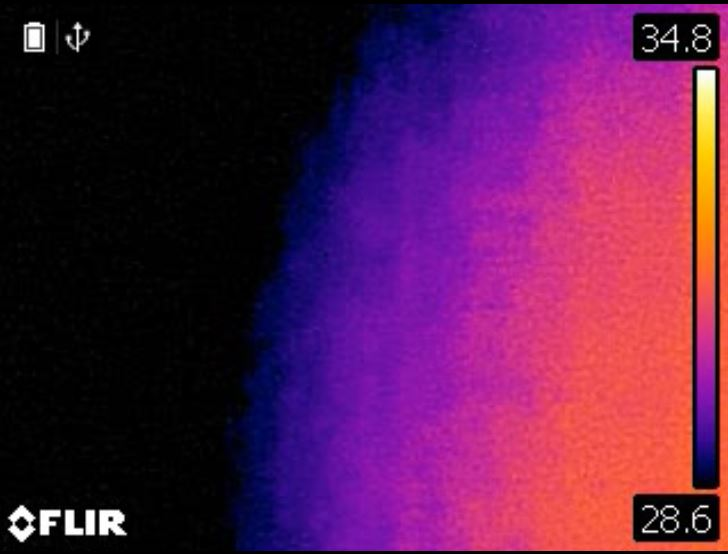
\includegraphics[width=.5\textwidth]{verifikasjon-test/Kamera/skyer3.JPG}
    \caption{Her kan vi se et bilde tatt med kameraet rettet mot kanten av en sky. Vi kan se at skyen, altså områdene med farge, gir en betydelig større utfordring når bildene skal filtreres.}
    \label{fig:verifikasjon:kamera_skyer}
\end{figure}

Det er usikkert hvordan systemet fungerer i andre værforhold som snø, regn og tåke, siden vi ikke ønsket å risikere å ødelegge lånt utstyr eller \todo{I tillegg til, eller bare bruke en av forklaringene} at disse værforholdene ikke var tilgjengelige under testing.
Derimot har FLIR funnet ut at ved sikt på under 300 meter ved elektromagnetisk stråling reiser like langt for IR-bølger som synlig lys \cite{tåke}.
Utfordringen ligger i refraksjon av elektromagnetiske bølger når de kommer i kontakt med regndråper eller snø \cite{refraksjon}.
Dette vil kunne føre til en mindre sannsynlighet for at strålingen fra fuglene  som skal observeres når fram til sensoren. I tillegg er det ikke usannsynlig at regn og snø kan feilaktig bli detektert av systemet som fugler. \todo{litt kronglete formuleringer i dette avsnittet. Skrive om litt}


\subsubsection{Kalibrering}\label{sec:verifikasjon:kamera:kalibrering}

Med jevne mellomrom kalibrerer kameraet seg. 
Kameraet er et kommersielt produkt, og programvaren vil justere kameraet for å gi større kontrast mellom de varme områdene i et bilde. 
Dette skjer oftere dersom varme objekter raskt forsvinner ut av bildet, eller dersom det er mulig å finne store kontraster som for eksempel når det er skyer. 
Dette er ugunstig ettersom at vi ikke ønsker at kameraet skal fremkalle varmesignaturer på denne måte. 
Når kameraet kalibreres oppstår det mønstre på skjermen, som vist i \autoref{fig:verifikasjon:kalibrering}, og dette er utvilsomt noe av det som ga store feil i form av falske positiver (registrering av fugler som ikke var tilstede). \todo{gi noen tall på antall feil}

En test som ble utført var å peke kameraet mot en fulg, slik at man lot kamereaet kalibrere seg. 
Bildene ville ofte gi tydelige kontraster mellom fugler og bakgrunn uavhengig om det var skyer eller ikke siden fuglene var mye varmere i kontrast til bakrunnen. 
Utfordringer oppsto når fulgen forsvann ut av synsfeltet til kameraet, og kameraet ville forsøke å kalibrere seg mot det nye motivet. Dersom det var skyer ville dette ofte gi output som i \autoref{fig:verifikasjon:kalibrering} etterfulgt av støyfulle bilder som i \autoref{fig:verifikasjon:kamera_skyer} som vi undersøkte i \autoref{sec:verifikasjon:kamera:værforhold}. 
Dette var et mer ubetydelig problem ved skyfri himmel, ettersom at den nye outputen ville bli som i \autoref{fig:verifikasjon:kamera_skyfri}.

\begin{figure}[H]
    \centering
    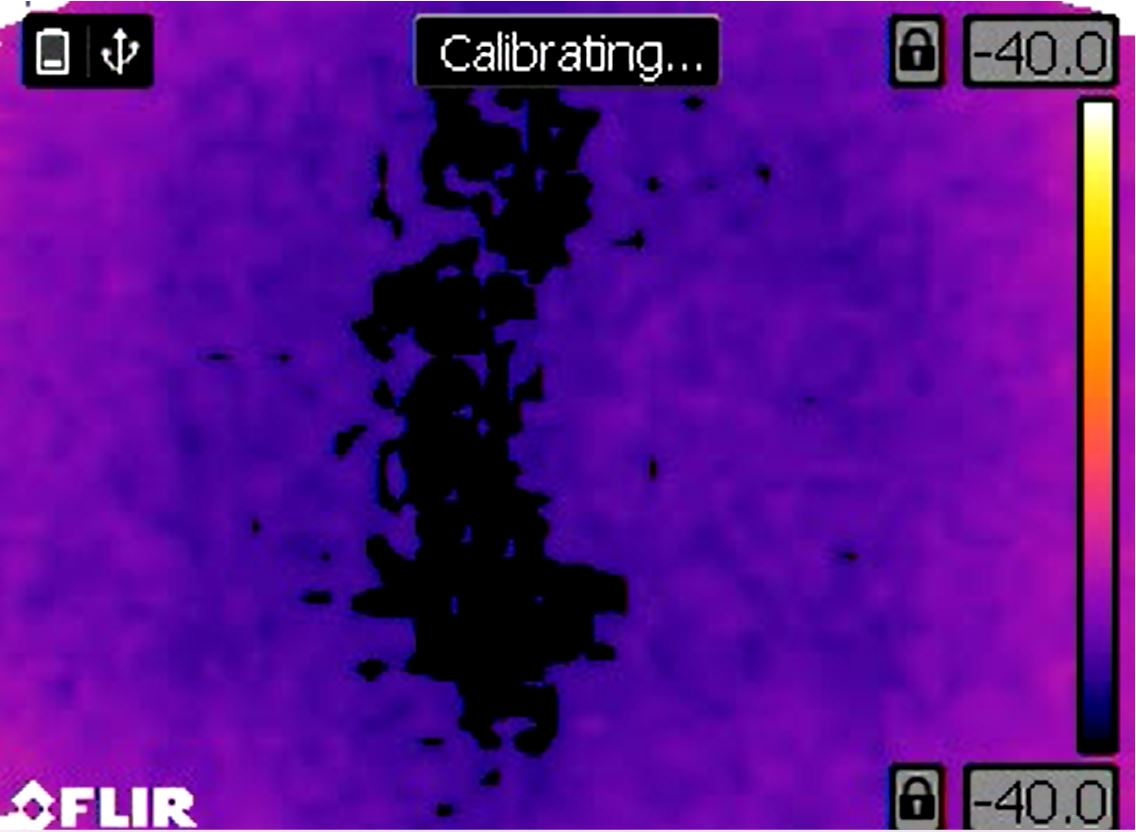
\includegraphics[width=.5\textwidth]{verifikasjon-test/Kamera/kalibrering.jpg}
    \caption{Et eksempel på hva som skjer når kameraet kalibreres.}
    \label{fig:verifikasjon:kalibrering}
\end{figure}
Når dette skjer vil mange blobs bli detektert i bildet, og det vil opprettes trackere for disse. Det vil føre til at programmet teller veldig mange fugler som ikke er der, i tillegg til at prosessoren ikke har nok prosessorkraft til å oppdatere alle trackerene.
\todo{Mulig forbedring med en ir-sensor hvor fokuset kan låses, slik at det ikke kalibrers av seg selv? Legges inn inn i kapittel om forbedringer?}


\subsection{Programvare}\label{sec:verifikasjon:programvare}

\subsubsection{Filtrering}\label{sec:verifikasjon:programvare:filtrering}

Skal teste litt med før jeg skriver denne her -> ludvik sitt ansvar i guess

Kommer litt bilder og tekst til eksempler som dette:

\begin{figure}[H]
    \centering
    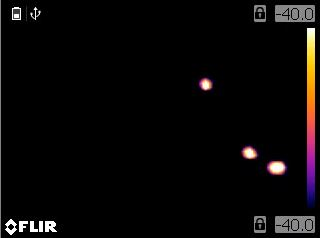
\includegraphics[width=.5\textwidth]{verifikasjon-test/Tracking_ex/org1.JPG}
    \caption{Org fra kamera.}
    \label{fig:verifikasjon:filtrering:1}
\end{figure}
\begin{figure}[H]
    \centering
    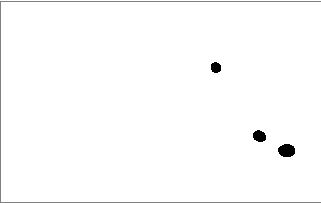
\includegraphics[width=.5\textwidth]{verifikasjon-test/Tracking_ex/filt1.JPG}
    \caption{Filtrering av org.}
    \label{fig:verifikasjon:filtrering:2}
\end{figure}

\subsubsection{Blob-deteksjon og tracking}\label{sec:verifikasjon:programvare:blob-detection_og_tracking}
I en testvideo med 20 fugler og skyfri himmel, var det to fugler systemet ikke klarte å oppdage. Det vil si at blob-deteksjon oppdaget 90\% av alle fuglene i videostrømmen. Av disse 18 fuglene som ble detektert klarte trackinga å følge 15 av fuglene helt til de forsvant ut av skjermen. På tre av fuglene mistet trackeren fuglen en gang, og startet en ny tracker. De tre fuglene ble altså telt to ganger hver. Det vil si at trackinga fungerte i 83\% av de tilfellene den fikk kjøre.

Det vil si at systemet telte 15 av 20 fugler, altså 75\% av fuglene, uten feil. Dette ligger innenfor systemkrav \idref{id:treffrate}. I to tilfeller telte den ikke fuglen som fløy i bildet og i tre tilfeller telte den fuglen to ganger. Det betyr at etter de 20 fuglene hadde flydd forbi, hadde 21 fugler blitt telt av systemet.

Trackinga har ikke blitt testet godt nok når det har vært overskyet, men dersom filtreringa klarer å fjerne bakgrunnen helt, vil trackinga fungere som på skyfri himmel. Om det derimot vil bli med forstyrrelser fra skyene i den filtrerte videostrømmen, vil trackinga få større problemer med å følge fuglene.

\todo{Nevne figurene i teksten}
\begin{figure}[H]
    \centering
    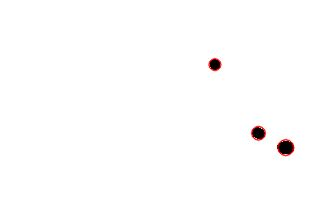
\includegraphics[width=.5\textwidth]{verifikasjon-test/Tracking_ex/blobs1.JPG}
    \caption{blob detection.}
    \label{fig:verifikasjon:blob:1}
\end{figure}
\begin{figure}[H]
    \centering
    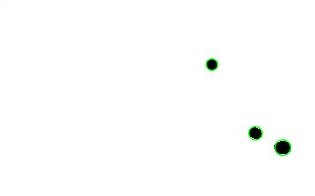
\includegraphics[width=.5\textwidth]{verifikasjon-test/Tracking_ex/track1.JPG}
    \caption{tracking.}
    \label{fig:verifikasjon:tracking:1}
\end{figure}

\subsection{Værstasjon}\label{sec:verifikasjon:telemetri}
Kommunikasjon mellom Raspberry Pi og de ulike sensorene er oppnådd, og sensorene sender ut fornuftig data. 

\subsection{Nettside og database}\label{sec:verifikasjon:nettside}

Fordi systemet ikke er testet i sin helhet over lengre tid ble databasen fylt med testdata. Denne dataen er generert slik at en kan se forskjell på dataen. Programmet som genererer testdataen ligger også i jolyu sin GitHub \cite{GitHub}. Nettsiden leser denne dataen og produserer grafer som visualiserer dataen på en fornuftig måte, og oppfyller derfor systemkrav \idref{id:nettside}. 

Overføring av data fra prosessorenhet er også testet ved å skrive værdata og telemetri til databasen. Dette fungerer også slik som det skal, og dermed oppfyller systemkrav \idref{id:eksternoverføring}.


\subsection{Systemet som en helhet}\label{sec:verifikasjon:helhet}
Systemkrav \idref{id:mål} og \idref{id:opensource} er oppnådd, siden systemet utfører oppgavene sine. Igjen så er dette gjort med testdata, siden systemet ikke er testet met ekte data som helhet.



\subsection{Koronatrøbbel}
\todo{skal subsec korona være med? må nok skrives om litt isåfall}
%Dette fikk vi ikke testet pga korona. eks alt sammen + vanntetting

Grunnet koronapandemien var det enkelte ting som var planlagt å teste, og som vanligvis ville vært mulig å teste, som ikke lot seg gjennomføre. Stengningen av campus gjorde at det ikke var mulig å 3d-printe boksen til elektronikken, slik at det ikke lot seg teste i hvilken grad denne er værbestandig, og heller ikke om den ellers utfører sine oppgaver godt. Det var heller ikke mulighet for å sette alle systemets strukturelle deler sammen, slik som å feste boks og sensorer til stativ. Det største problemet var at testing av hele systemet satt sammen ble umulig, da utstyr ble spredt mellom gruppemedlemmer for å kunne fortsette arbeid hver for seg. Dette gjør at testing av systemkrav \idref{id:IPrating} ikke har vært mulig testing. Systemkrav \idref{id:størrelse} er gjennomført i den grad at boksen er designet, men ikke 3D-printet. 


